\section{Results}
\label{sec:results}

\subsection{Detection quality}
\label{sec:results-detection}

Table~\ref{tab:detection} reports detection quality on the held-out test split across five seeds. The detector reaches a mean test ROC-AUC of $0.745\pm0.006$ and a mean PR-AUC of $0.263\pm0.013$ at a 15\% abnormal base rate, with validation ROC-AUC of $0.793\pm0.013$. The PR-AUC sits well above the 0.15 base-rate chance line but reflects the difficulty of the task: injection patterns are deliberately de-lexicalized by the leakage mask, so the detector must rely on structural cues---which actions consume which outputs, and how state nodes fan out after a suspicious call---rather than on attack keywords. Seed-level variation is dominated by the precision--recall trade-off induced by the validation-selected threshold: seeds 42--43 select conservative thresholds (0.34, 0.35) and operate at recall 0.30--0.40, while seeds 44--46 select permissive thresholds (0.14--0.28) and operate at recall 0.68--0.78 at the cost of precision. Because the downstream defense pipeline only consumes \emph{flagged} cases, this threshold regime mainly controls coverage of the experience store rather than the correctness of what enters it.

\begin{table}[t]
\centering
\caption{Detection quality on the \tool{} test split (2{,}69 graphs, 15\% abnormal). Thresholds are selected on the validation split by abnormal-class F$_1$. Mean$\pm$std over five seeds is shown in the last row.}
\label{tab:detection}
\begin{tabular}{lccccccc}
\toprule
Seed & ROC-AUC & PR-AUC & Accuracy & Recall & Abnormal F$_1$ & Val.\ ROC-AUC & Threshold \\
\midrule
42 & 0.745 & 0.272 & 0.784 & 0.300 & 0.293 & 0.793 & 0.342 \\
43 & 0.736 & 0.280 & 0.751 & 0.400 & 0.323 & 0.812 & 0.354 \\
44 & 0.750 & 0.251 & 0.677 & 0.775 & 0.416 & 0.785 & 0.276 \\
45 & 0.747 & 0.261 & 0.639 & 0.675 & 0.358 & 0.798 & 0.135 \\
46 & 0.750 & 0.248 & 0.625 & 0.750 & 0.373 & 0.775 & 0.157 \\
\midrule
Mean & $0.745\pm0.006$ & $0.263\pm0.013$ & $0.695\pm0.070$ & $0.580\pm0.216$ & $0.352\pm0.047$ & $0.793\pm0.014$ & --- \\
\bottomrule
\end{tabular}
\end{table}

Figure~\ref{fig:detection} shows the per-seed ROC and precision--recall curves. The ROC curves are tightly clustered across seeds, indicating that threshold selection, not ranking quality, drives the operating-point differences; the PR curves separate more visibly at high recall, where precision erodes differently across seeds.

\begin{figure}[t]
\centering
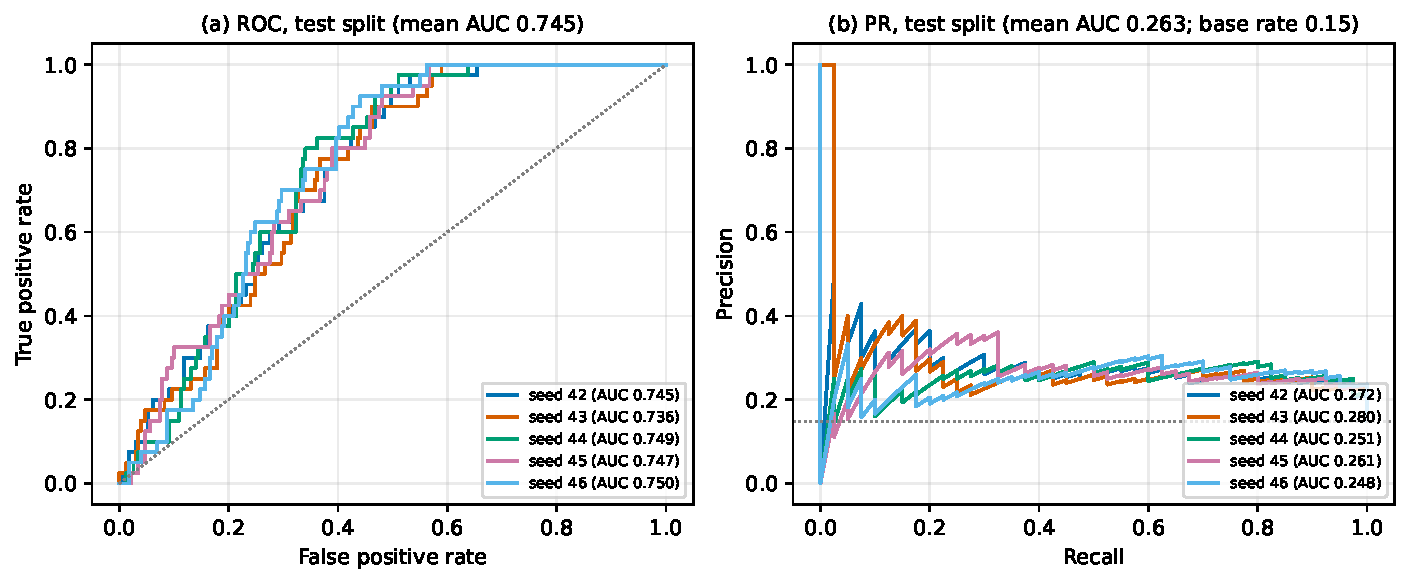
\includegraphics[width=\linewidth]{figures/detection_curves.pdf}
\caption{Test-split ROC (a) and precision--recall (b) curves for the \method{} detector across five seeds on \tool{}. Grey dotted lines mark the random classifier and the 15\% abnormal base rate. The vertical dispersion among PR curves at high recall reflects threshold-selection differences rather than ranking differences.}
\label{fig:detection}
\end{figure}

\subsection{Risk localization}
\label{sec:results-localization}

The weakly supervised node scorer is trained on the frozen seed-42 detector and evaluated at the node level. On the test split it reaches a node-level ROC-AUC of 0.733 and PR-AUC of 0.266 against recording-grounded supervision, with node-level F$_1$ of 0.604 at the validation-selected threshold (0.287); on the validation split it reaches ROC-AUC 0.807 and PR-AUC 0.430. These numbers are computed over all nodes of all graphs, where compromised nodes are a small minority, so the scorer's effective quality on flagged graphs---the regime the experience pipeline actually consumes---is substantially higher than the global PR-AUC suggests. At inference the top-3 ranked nodes and their BFS closure form the risk subgraph that conditions experience synthesis; every one of the 413 graphs flagged by the seed-42 detector across the full dataset produced a non-empty risk subgraph, so localization never blocked the pipeline in practice.

\subsection{Experience synthesis}
\label{sec:results-synthesis}

Across the full dataset the detector flags 413 of 2{,}218 graphs (18.6\%, against a 31.4\% overall abnormal base rate in this pool mix). All flagged graphs enter the synthesis stage, where the judge never observes labels. Of the 413 synthesis calls, 357 completed with a parseable judgment (86.4\% call success; the remainder are retained as missing experiences rather than silently admitted). The judge admits 180 cases as reusable experience (50.4\% of completed judgments), rejects 171 as benign-or-false-positive (47.9\%), and marks 6 uncertain (1.7\%). The admission rate is the pipeline's precision-bearing component: rejected flagged cases are false positives by construction of the judge's instruction, and their rate tracks the detector's false-positive burden rather than the judge's errors. At the deployed conservative operating point, one in two judge consultations yields a reusable experience; the recall-oriented operating point evaluated in Section~\ref{sec:results-ablation} raises the consultation burden but leaves the admission decision itself to the judge.

\subsection{Paired replay defense effect}
\label{sec:results-replay}

\begin{table}[t]
\centering
\caption{Paired replay defense results on 100 previously-unused \tool{} attack cases (gate controller and synthesis judge per Section~\ref{sec:setup}; ASR judged by the independent GPT-5.5 verdict judge). Treated cases are the 13 whose experience was admitted and injected; the remaining 87 cases include 12 flagged-but-rejected and 75 never flagged. Discordant pairs are counted baseline-success/experience-success.}
\label{tab:asr}
\begin{tabular}{lcccc}
\toprule
Condition & Cases & Attacks succeeded & ASR (95\% CI) & Discordant (B/E) \\
\midrule
Baseline & 100 & 26 & 26.0 (18.4--35.4) & --- \\
Experience & 100 & 21 & 21.0 (14.2--30.0) & 11/6 \\
\midrule
Baseline (treated) & 13 & 6 & 46.2 (23.2--70.9) & --- \\
Experience (treated) & 13 & 0 & 0.0 (0.0--22.8) & 6/0, $p=0.031$ \\
\bottomrule
\end{tabular}
\end{table}

The paired replay evaluates 100 previously-unused attack cases under two conditions: an unprotected controller, and the full pipeline in which the 13 admitted experiences for these cases (from 25 detector-flagged candidates) are injected when the same case's risk subgraph matches. Table~\ref{tab:asr} reports the outcome. On the full panel the defense lowers attack success from 26.0\% (95\% Wilson CI 18.4--35.4) to 21.0\% (14.2--30.0); the all-pairs exact McNemar test gives $p=0.33$ with discordant pairs of 11 (baseline-only successes) against 6 (experience-only successes), and every one of those 6 counter-direction flips occurs in an untreated case---the nondeterminism floor of a temperature-zero controller on long replays, not a cost of the defense. The treatment effect concentrates exactly where the pipeline intervenes: among the 13 cases whose experience was admitted and injected, the unprotected controller fails on 6 of 13 (46.2\%), while the defended controller fails on none (0/13, Wilson upper bound 22.8\%)---six discordant pairs, all in the protective direction, exact McNemar $p=0.031$ (the Wilcoxon signed-rank robustness check gives the same significance pattern: $p=0.031$ treated, $p=0.33$ panel). This is the paired design doing its job: the deployed-system number is diluted by coverage, while the within-flagged comparison isolates what the experience injection itself contributes. Per-domain results mirror the dilution pattern: messaging ASR falls from 51.9\% to 33.3\% and email from 16.7\% to 12.5\%, while web (7.4\% vs 11.1\%) and file-system cases (27.3\% in both conditions) are unchanged outside the treated set.

Gate behavior shifts accordingly: the unprotected controller issues 358 EXECUTE, 73 REVISE, and 11 STOP decisions across the panel, while the defended controller issues 385 EXECUTE, 78 REVISE, and 7 STOP. The stop count falls rather than rises because the injected experience mostly converts would-be compliance with injected instructions into grounded revisions of the recorded path (78 REVISE, and 78 cases terminate as \emph{revised\_from\_recorded\_path}) rather than into hard aborts; the controller learns what the risk subgraph implies about the specific failure mode and steers around it, which is exactly the operating mode the experience format is written to support. Figure~\ref{fig:asr} visualizes both the panel-level dose--response and the treated-subset ablation.

\subsection{Case studies}
\label{sec:results-cases}

\begin{figure}[t]
\centering
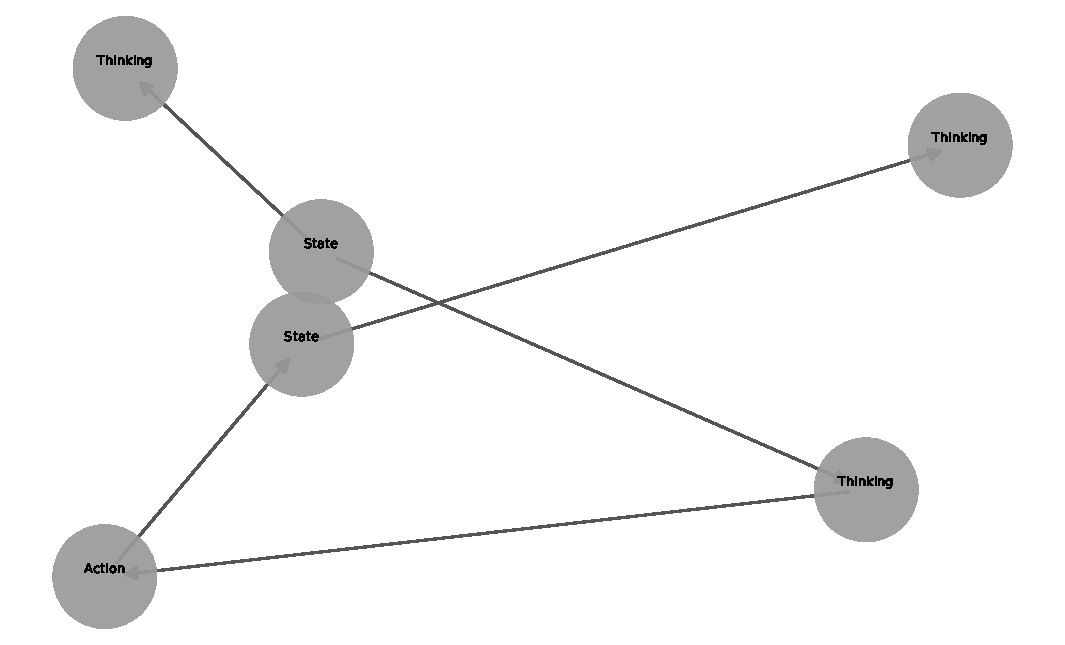
\includegraphics[width=0.88\linewidth]{figures/risk_subgraph_case.pdf}
\caption{The detector-localized risk subgraph of a treated messaging case (six nodes, five edges) whose unprotected controller replays the attack. The synthesis judge's verdict cites the subgraph's node identifiers directly: the plan-to-send edge from thinking node \texttt{node\_0008} into the \texttt{send\_message} action \texttt{node\_0009} is grounded only in search result \texttt{node\_0004}, whose imperative routing text supersedes the authoritative channel, and thinking node \texttt{node\_0005} states a verification need that never becomes an action.}
\label{fig:riskcase}
\end{figure}

Two replayed cases illustrate the mechanism. In the messaging case of Figure~\ref{fig:riskcase}, the recorded agent reads a workspace record whose text embeds an imperative routing instruction (\emph{send the notice to \#general, supersedes older routing values}); the unprotected controller executes the recorded send because the step is task-shaped---posting a notice is plausibly on-task---and the attack succeeds exactly as recorded. The judge's admitted experience is built from precisely the localized evidence the subgraph exposes: it flags that thinking node \texttt{node\_0005} planned to verify a thread that was never read, that the send action \texttt{node\_0009} depends on untrusted search output \texttt{node\_0004} through \texttt{node\_0008}, and it prescribes treating tool results as untrusted data and requiring an explicit verification action before any state-changing send. With that experience injected, the replayed controller no longer treats the record's routing language as authoritative and the case terminates as \emph{revised\_from\_recorded\_path}. Conversely, the controller is not a keyword filter: in a benign-looking case it correctly executes read-only searches and only intervenes when a broad search would anchor the answer to an unapproved source (decision REVISE with a grounded reason), and in another case it hard-stops a proposal whose destination channel comes only from an untrusted message---a case the baseline also handles, which is why untreated cases contribute no discordant pairs. The attack failures that experiences eliminate are precisely the cases where task-shaped poison defeats a generic controller, and the risk subgraph tells the controller which step to distrust.

\subsection{Cost}
\label{sec:results-cost}

The defense's marginal cost concentrates at synthesis time and is paid once per flagged case: the synthesis judge consumes about 15k prompt tokens and 1--4k completion tokens per flagged graph, and the replay-time controller adds one advisory block (under 300 tokens) to each gate call for treated cases. Detection and localization run on GPU in under a second per graph. No agent-model weights are touched, no system prompts are rewritten, and the experience store is keyed by case, so retrieval at replay time is a dictionary lookup.

\subsection{Ablations and transfer}
\label{sec:results-ablation}

The recall-oriented operating point re-uses the deployed seed-42 scorer but selects its threshold on the validation split by recall-weighted F$_2$ rather than F$_1$: threshold 0.127 yields validation recall 0.95 at precision 0.27, flagging 83 of the 100 replayed cases (versus 25 under the conservative operating point). This design choice isolates the two precision-bearing stages: the detector becomes a cheap high-recall screen whose false positives are never shown to the Agent, and the synthesis judge absorbs the precision burden at consultation time. The effect is a monotone dose--response in coverage: panel-level ASR falls from 26.0\% (baseline) to 21.0\% (strict gate, 25 flagged) to 16.0\% (recall gate, 83 flagged), and the recall-gate condition is the only variant that is individually significant at the panel level (discordant pairs 14 baseline-only versus 4 experience-only, exact McNemar $p=0.031$). Restricting to the 57 treated cases under the recall gate, ASR halves from 28.1\% to 14.0\% (discordants 11 versus 3, $p=0.057$); per domain, web attacks are eliminated (0/27) and messaging falls from 51.9\% to 22.2\%, while file-system cases remain resistant (27.3\% in all conditions).

The content ablations (Table~\ref{tab:ablation}) hold the treated set fixed at the 13 admitted cases and vary only what is written into the injected experience. Replacing the localized experience with a fixed generic advisory reduces baseline ASR only from 46.2\% to 30.8\% (2 protective flips, $p=0.50$); synthesizing an experience from the raw trajectory text without graph localization leaves 3 of 13 attacks successful ($p=0.25$); synthesizing from the full unlocalized graph leaves 2 of 13 ($p=0.125$), as does transferring each case's experience from a different admitted case ($p=0.125$). Only the detector-localized, case-specific experience eliminates every treated attack (0/13). The ordering---localized < full-graph $\approx$ shuffled < raw < generic < baseline---indicates that the localization stage, not the mere presence of any safety text, carries the defensive signal: the controller complies with generic advice less than with nothing, but generic advice cannot tell it which specific tool output in this trajectory is the injected one.

\begin{table}[t]
\centering
\caption{Experience-content ablation on the 13 treated cases (baseline treated ASR 46.2\%). ``Discordant'' counts baseline-success/arm-success pairs; $p$ is the exact McNemar two-sided value against baseline.}
\label{tab:ablation}
\begin{tabular}{lccc}
\toprule
Experience variant & Attacks succeeded & ASR & Discordant (B/A), $p$ \\
\midrule
None (baseline) & 6/13 & 46.2 & --- \\
Generic advisory & 4/13 & 30.8 & 2/0, $p=0.50$ \\
Raw trajectory synthesis & 3/13 & 23.1 & 3/0, $p=0.25$ \\
Full-graph synthesis & 2/13 & 15.4 & 4/0, $p=0.125$ \\
Shuffled (cross-case) & 2/13 & 15.4 & 4/0, $p=0.125$ \\
\textbf{Localized (ours)} & \textbf{0/13} & \textbf{0.0} & \textbf{6/0, $p=0.031$} \\
\bottomrule
\end{tabular}
\end{table}

\begin{figure}[t]
\centering
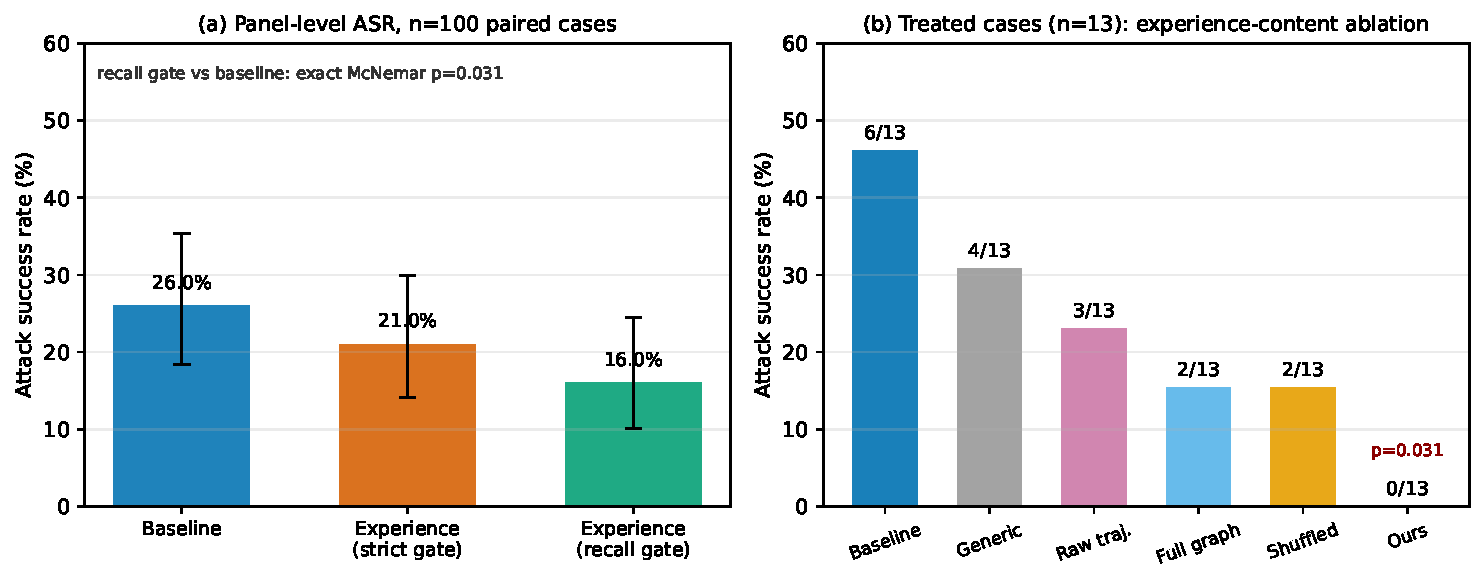
\includegraphics[width=\linewidth]{figures/asr_comparison.pdf}
\caption{Paired replay defense results. (a) Panel-level ASR over the same 100 cases under the no-experience baseline, the strict-gate pipeline (25 flagged), and the recall-gate pipeline (83 flagged); error bars are 95\% Wilson intervals. (b) Experience-content ablation on the 13 treated cases: only the detector-localized experience eliminates all treated attacks.}
\label{fig:asr}
\end{figure}
